\documentclass{sintefbeamer}
\usepackage[UTF8]{ctex}
\setCJKmainfont[
  UprightFont={C:/Windows/Fonts/simsun.ttc},
  % BoldFont={C:/Windows/Fonts/Songti SC.ttf}
  BoldFont={C:/Users/LIMINGNING/Downloads/Songti SC.ttf}
]{Songti SC}
\usepackage{booktabs}
\usepackage{array}
\usepackage{tabularx}
\usepackage{graphicx}
\usepackage{hyperref}
\usepackage{tikz}
\usetikzlibrary{arrows.meta, positioning, shapes.geometric}

\renewcommand{\strtoc}{目录}
\newcolumntype{B}[1]{>{\bfseries\raggedright\arraybackslash}p{#1}}
\newcolumntype{P}[1]{>{\raggedright\arraybackslash}p{#1}}
\newcolumntype{Y}{>{\raggedright\arraybackslash}X}
\newcommand{\tablebody}{\footnotesize\renewcommand{\arraystretch}{1.16}}

\title{面向开放域问答的\\工具调用智能体设计与优化}
\subtitle{本科毕业设计开题报告}
\author[李明柠]{\texorpdfstring{%
  \begin{tabular}{@{}l@{}}
    李明柠 \quad 2023311423\\[0.3em]
    指导教师：陈科海
  \end{tabular}%
}{李明柠 2023311423 指导教师：陈科海}}

\date{2026年4月}
\titlebackground{images/background}

% 覆盖模板默认的极小 block 字号；正文保持 small，避免三栏页过挤
\setbeamerfont{block title}{series=\bfseries\centering, size=\normalsize}
\setbeamerfont{block body}{size=\small}

\newcommand{\kw}[1]{\textbf{\textcolor{sintefblue}{#1}}}
\newcommand{\muted}[1]{\textcolor{airforceblue}{#1}}
\newcommand{\tinyurl}[1]{\texttt{\scriptsize #1}}
\newcommand{\tightlist}{\setlength{\itemsep}{0.45em}\setlength{\parskip}{0pt}}
\newcommand{\smalltag}[1]{%
  \tikz[baseline=(x.base)] \node[draw=sintefblue, rounded corners=1.5pt,
  inner xsep=4pt, inner ysep=1.5pt, line width=.45pt, text=sintefblue,
  font=\footnotesize] (x) {#1};%
}
\newcommand{\metric}[2]{%
  \begin{minipage}[t]{0.22\textwidth}
    \centering
    {\Large\bfseries\textcolor{sintefblue}{#1}}\\[-0.1em]
    {\scriptsize #2}
  \end{minipage}
}
\newcommand{\researchbox}[2]{%
  \fcolorbox{sintefblue}{white}{%
    \begin{minipage}[t][2.05cm][t]{0.43\textwidth}
      {\small\kw{#1}}\par\vspace{0.35em}
      {\scriptsize #2}
    \end{minipage}%
  }%
}

\begin{document}

\maketitle

% \begin{frame}{目录}{\,}
%   \tableofcontents[hideallsubsections]
% \end{frame}

\section{背景与意义}

% \begin{frame}{汇报主线：从问题到验证}
%   \begin{columns}[T]
%     \begin{column}{0.47\textwidth}
%       \begin{block}{为什么做}
%         开放域问答经常涉及最新事实、长尾实体和多跳关系，单靠模型参数记忆难以稳定回答。
%       \end{block}
%       \vspace{0.45em}
%       \begin{block}{问题在哪}
%         现有检索增强方法常见问题是触发不稳、查询不准、网页证据噪声大和调用成本不可控。
%       \end{block}
%     \end{column}
%     \begin{column}{0.47\textwidth}
%       \begin{block}{怎么解决}
%         围绕“何时搜、搜什么、怎么用”，设计检索触发、查询改写、证据压缩和预算控制模块。
%       \end{block}
%       \vspace{0.45em}
%       \begin{block}{怎么验证}
%         通过公开数据集与自建问题集，对准确性、检索有效性、调用效率和稳定性进行对比评测。
%       \end{block}
%     \end{column}
%   \end{columns}
%   \vspace{0.7em}
%   \centering
%   \kw{答辩陈述重点：本课题解决的是外部信息获取链路不可控的问题。}
% \end{frame}

\begin{frame}{课题背景：开放域问答需要外部知识}
  \centering
  \vspace{0.8em}
    \makebox[\textwidth][c]{%
      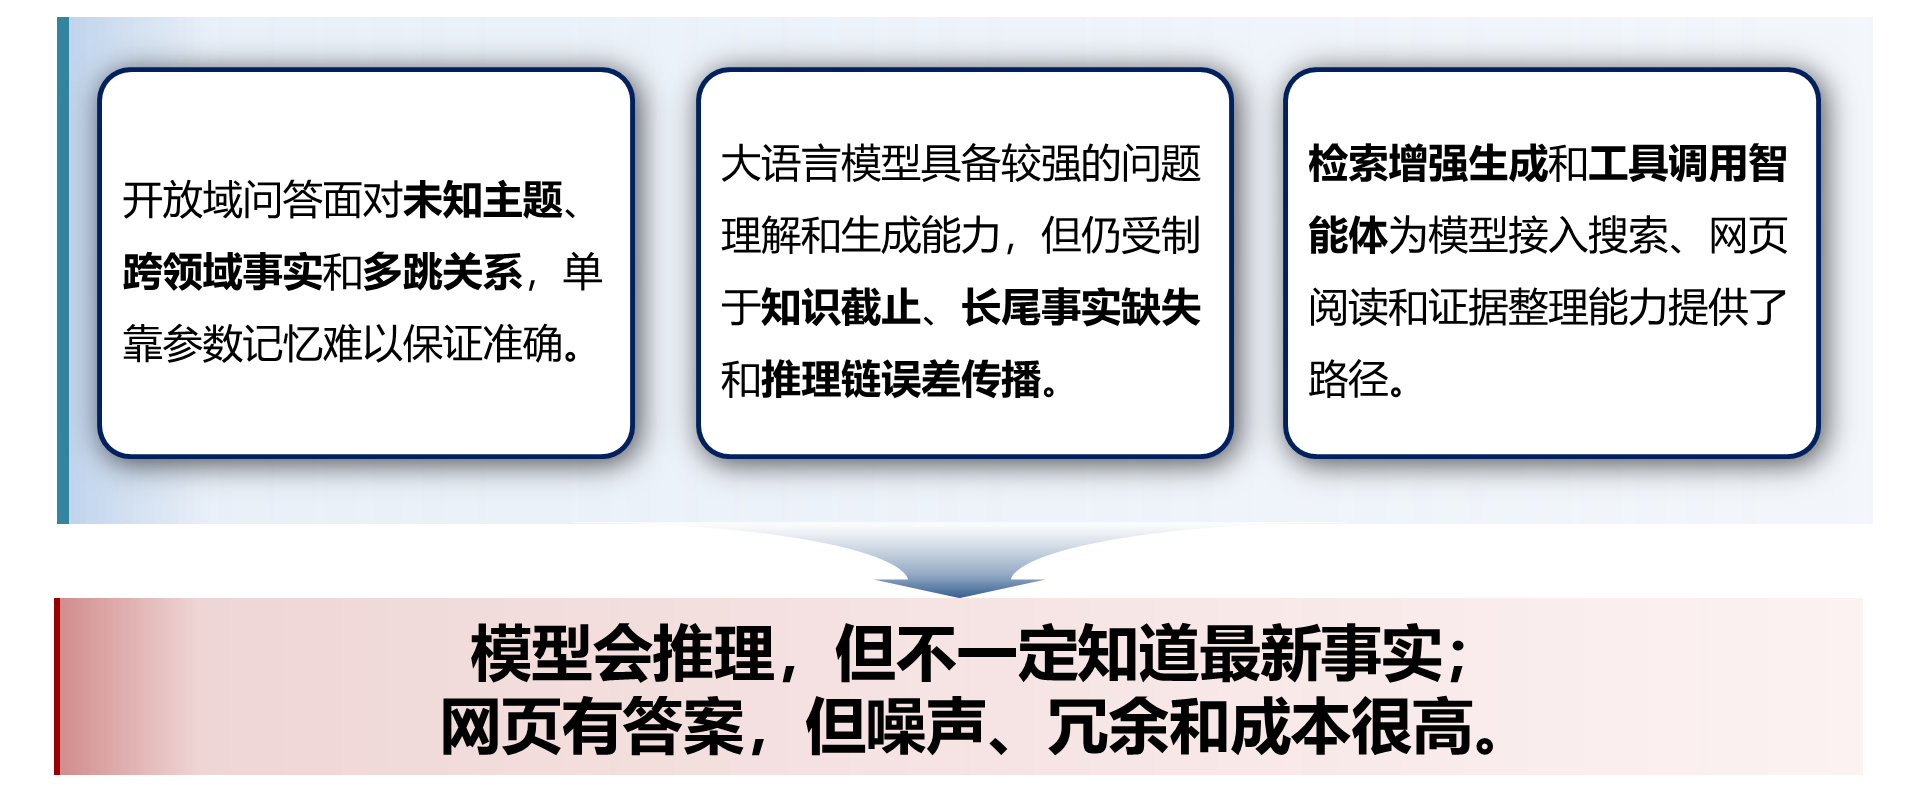
\includegraphics[
        width=1.08\textwidth,
        height=1.08\textheight,
        keepaspectratio
      ]{images/课题背景.png}%
    }
  % \centering
  % \vfill
  % \makebox[\textwidth][c]{%
  %   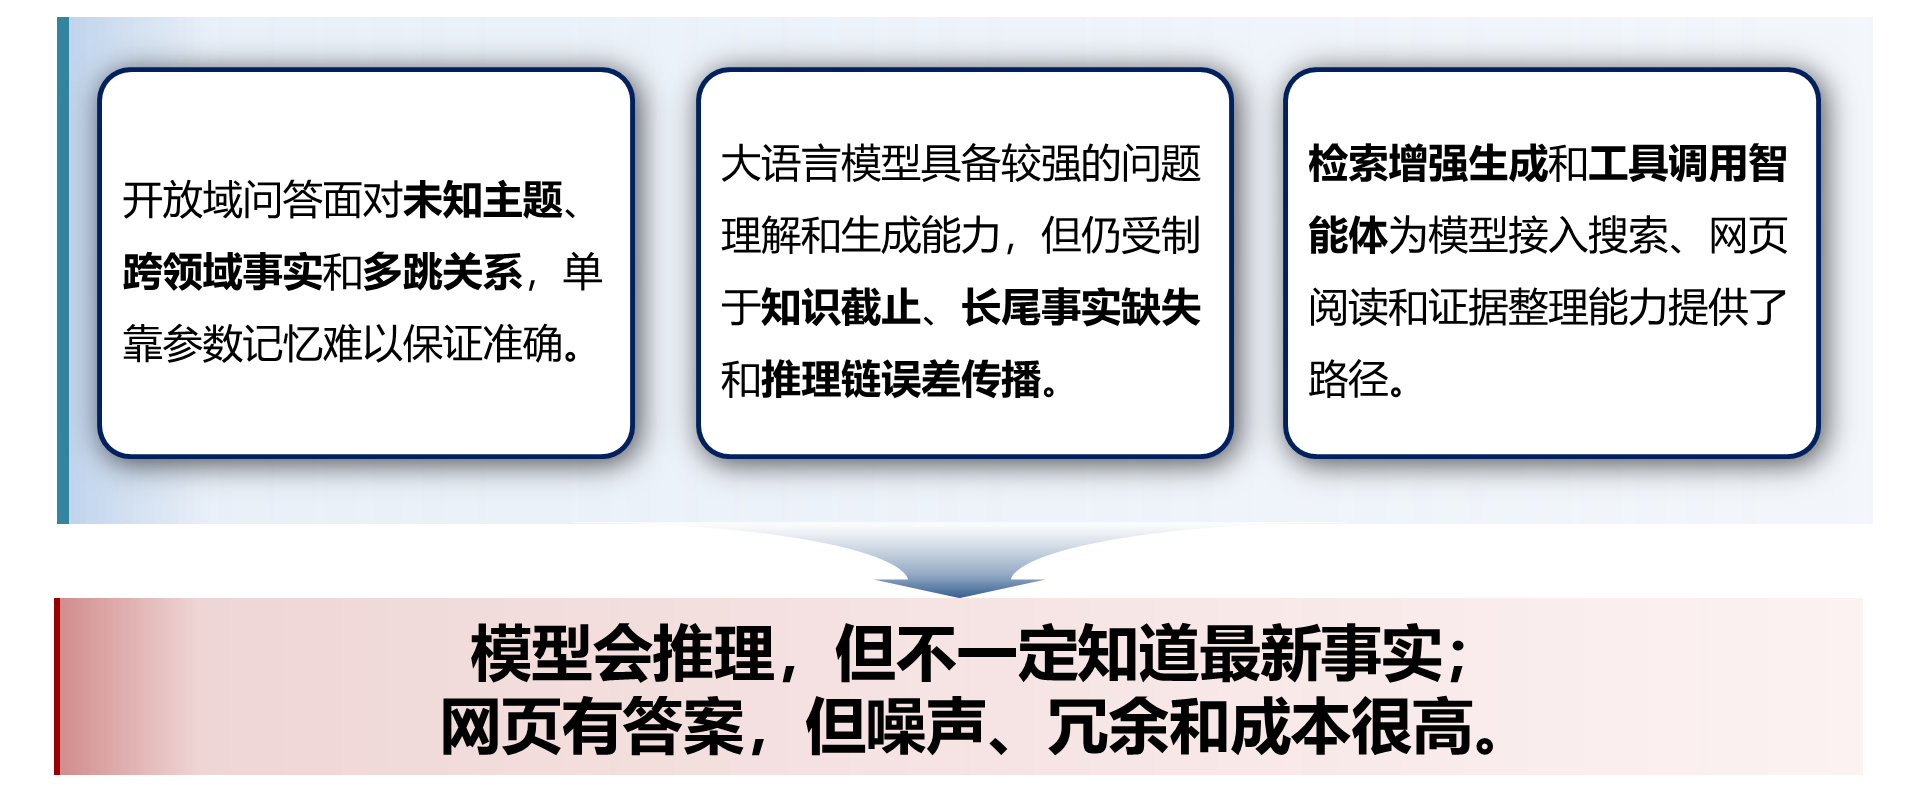
\includegraphics[
  %     width=1.08\textwidth,
  %     height=0.9\textheight,
  %     keepaspectratio
  %   ]{images/课题背景.png}%
  % }
  % \vfill
\end{frame}

% 这一页主要说明课题背景。开放域问答和普通问答不同，它的问题范围不固定，可能涉及不同领域、最新信息、冷门实体和多跳关系。因此，大模型只依赖训练阶段学到的参数记忆是不够的。

% 然后展开三个问题：

% 第一，知识有时效性。比如近期新闻、论文、产品信息、赛事结果等内容会不断变化，模型内部知识可能过时。
% 第二，长尾事实容易缺失。对于冷门人物、小众机构、具体网页信息，模型训练语料中覆盖不足，容易答错。
% 第三，多跳问题需要中间事实。模型需要先查到若干中间信息，再综合推理。如果中间事实错了，最终答案也会错。

% 然后引出你的课题：

% 所以开放域问答系统需要引入外部知识，尤其是网页检索和网页内容读取。我的课题就是在这个背景下，研究大模型智能体如何调用网页检索工具，并把检索到的网页信息整理成可用于回答的证据。

% 最后一句收束：

% 简单说，就是让模型不是凭记忆硬答，而是在需要的时候会查网页，并且能把查到的信息用好。

\begin{frame}{研究意义与实施意义}
  \centering
  \vspace{0.8em}
    \makebox[\textwidth][c]{%
      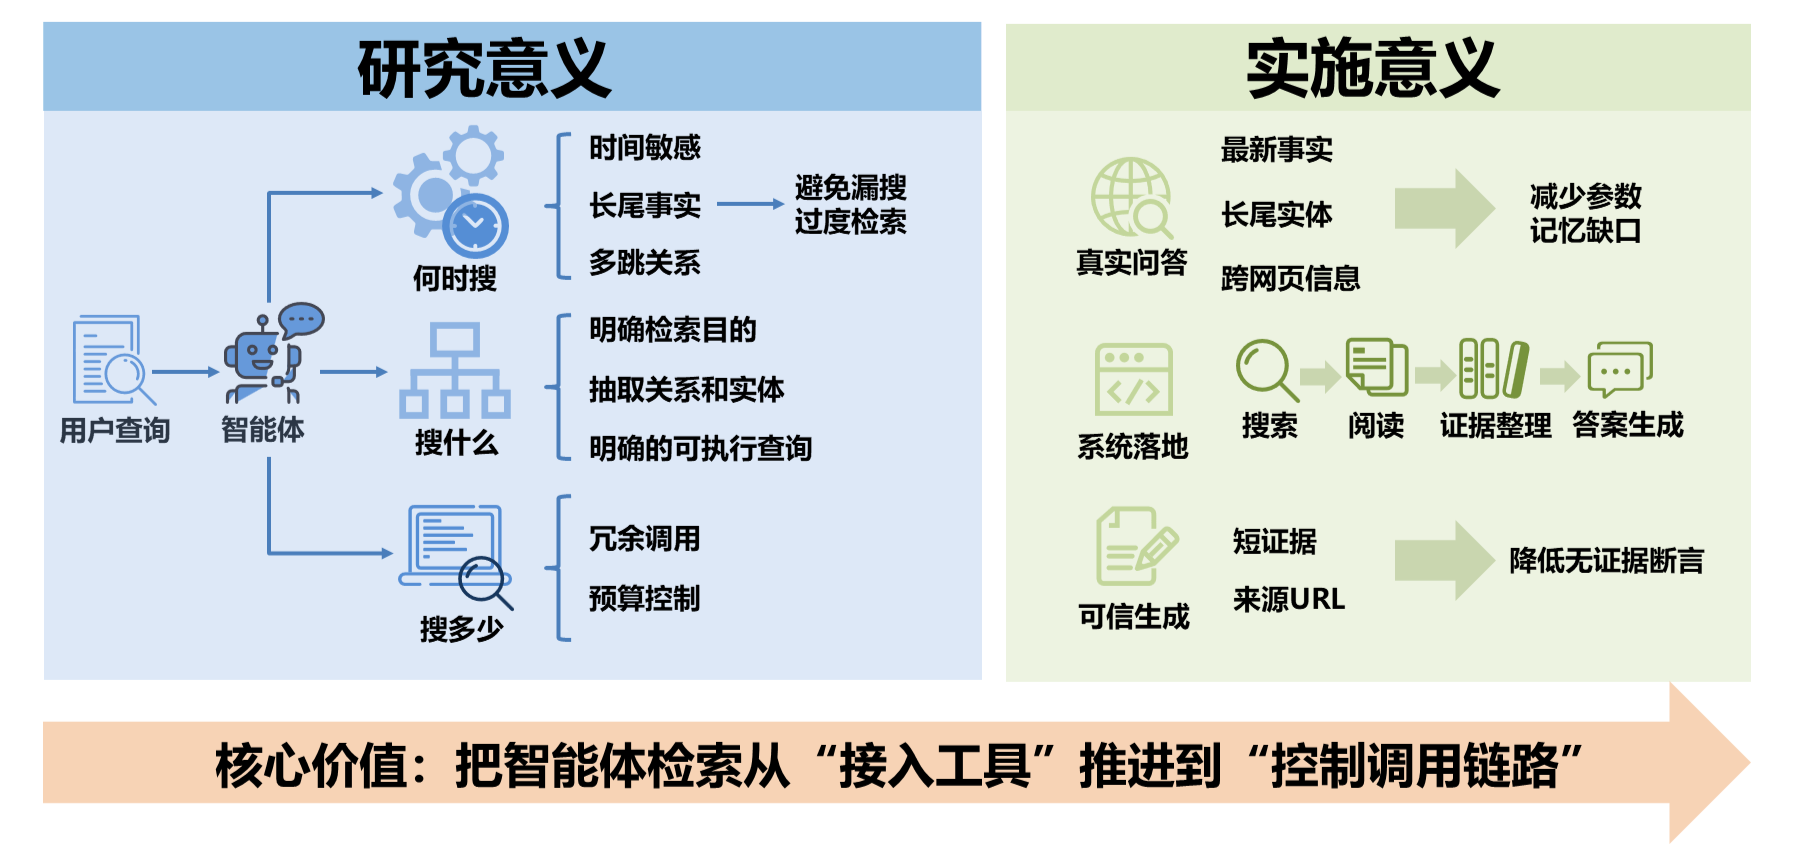
\includegraphics[
        width=1.08\textwidth,
        height=1.08\textheight,
        keepaspectratio
      ]{images/研究意义.png}%
    }
\end{frame}

% 研究意义主要体现在方法层面。当前很多系统已经可以接入搜索工具，但真正影响效果的是工具调用链路是否可控，也就是：什么时候搜、搜什么、搜多少。如果检索触发不稳定，就会出现简单问题过度检索，复杂问题漏检；如果查询生成质量不高，就很难召回关键网页；如果没有预算控制，多轮搜索会带来较高的延迟和成本。因此，本课题研究的是网页检索工具调用链路优化问题。

% 再讲实施意义：

% 实施意义主要体现在系统层面。本课题会实现一个面向开放域问答的网页检索智能体原型，跑通查询生成、外部检索、网页内容读取、证据整理和答案生成流程。这样系统不仅能调用网页获取外部知识，还能记录来源、整理短证据，并从准确性、检索有效性、调用次数和响应时间等指标上进行评测。

% 最后总结：

% 所以，研究意义是分析和优化网页检索工具调用机制；实施意义是做出一个可运行、可评测的开放域问答智能体原型。

\section{研究现状}

\begin{frame}{相关研究脉络}
  % \tablebody
  % \begin{tabularx}{\textwidth}{B{2.4cm}YP{4.0cm}}
  %   \toprule
  %   方向 & 代表思路 & 启示与不足 \\
  %   \midrule
  %   检索增强生成 & RAG 在生成前引入外部文档，缓解模型知识不足 & 典型流程多为一次性检索，难覆盖多跳中间事实 \\
  %   \addlinespace
  %   智能体工具调用 & WebGPT、ReAct、Self-Ask、IRCoT 等将搜索/阅读嵌入推理过程 & 能动态补充信息，但容易出现重复搜索、查询过宽和无关网页干扰 \\
  %   \addlinespace
  %   网页检索增强推理 & Search-R1、Search-o1、WebThinker 等强调多轮搜索、网页阅读和证据整合 & 真实网页存在长文本噪声、正文抽取失败和调用成本控制问题 \\
  %   \bottomrule
  % \end{tabularx}
  \centering
  \vspace{0.8em}
    \makebox[\textwidth][c]{%
      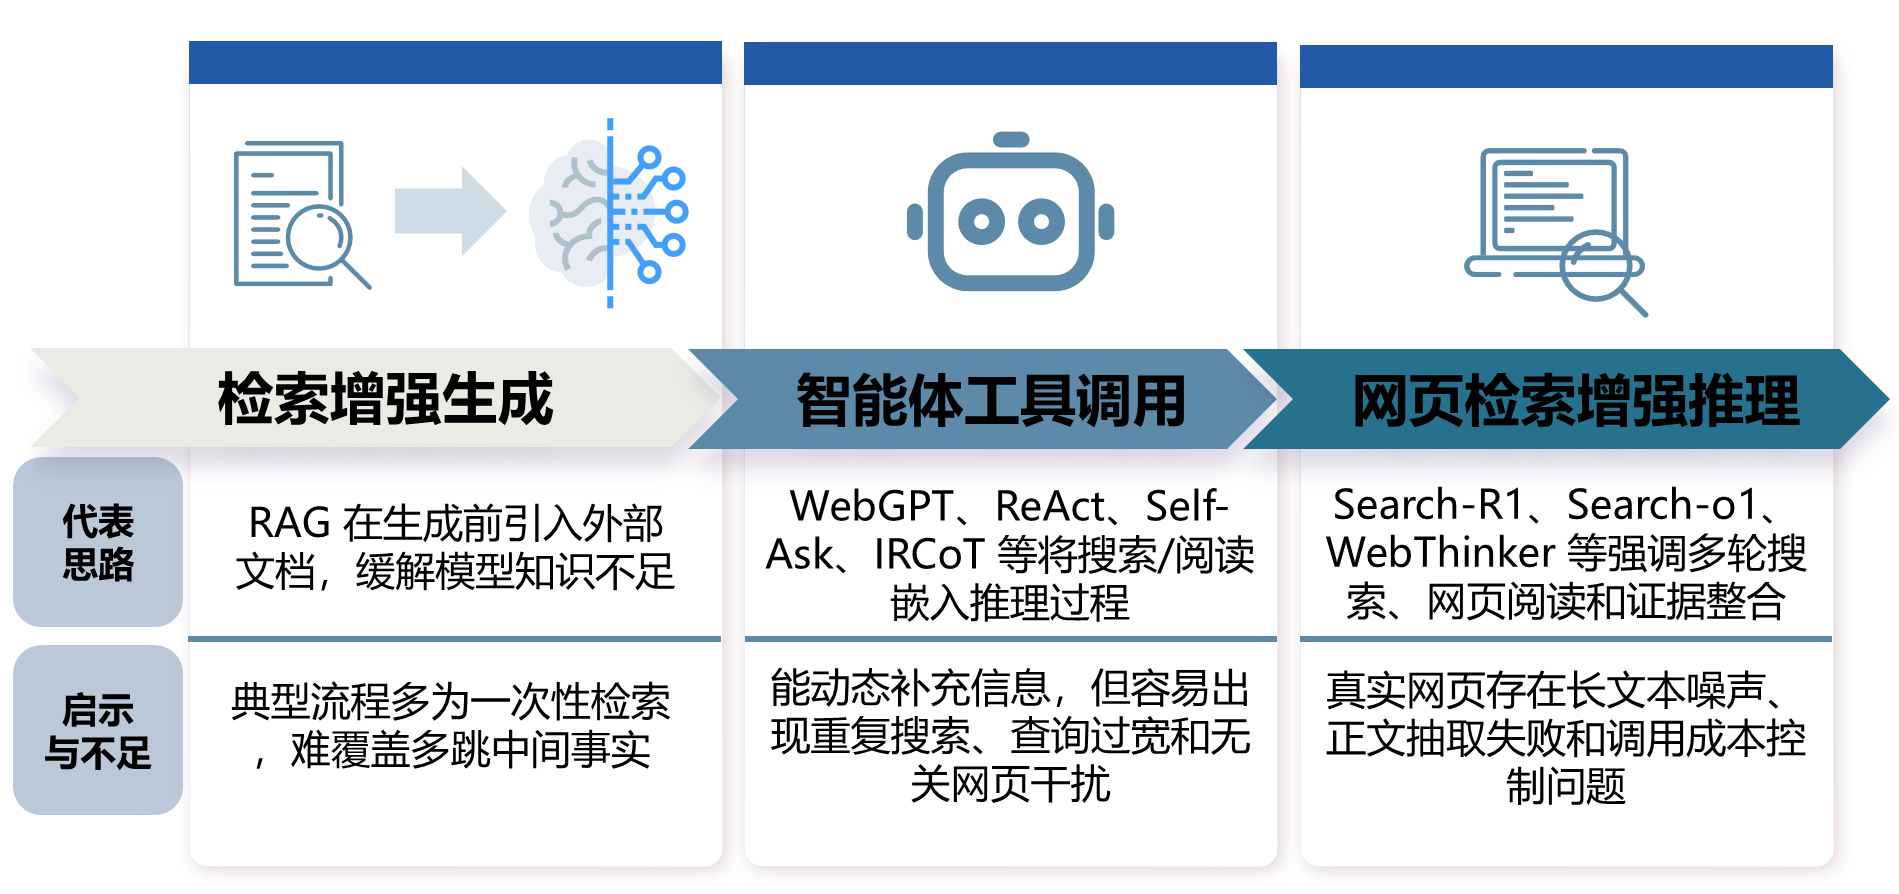
\includegraphics[
        width=1.08\textwidth,
        height=1.08\textheight,
        keepaspectratio
      ]{images/相关研究脉络.png}%
    }
\end{frame}

% 这一页主要梳理和本课题相关的研究脉络。我把相关工作分成三类。

% 第一类是检索增强生成，也就是 RAG。它的核心思路是在模型生成前引入外部文档，用来缓解大模型知识不足的问题。RAG 对开放域问答很重要，但典型流程通常是对原始问题做一次性检索，然后把 Top-K 文档交给模型，因此在多跳问题中，往往难以覆盖后续推理过程中才出现的中间事实。

% 第二类是智能体工具调用，例如 WebGPT、ReAct、Self-Ask 和 IRCoT。这类方法把搜索、阅读等动作嵌入推理过程，让模型可以在解题过程中动态补充外部信息。相比固定 RAG，它更灵活，但也带来新问题，比如什么时候搜索不稳定、查询可能过宽、重复搜索较多，以及网页内容可能干扰推理。

% 第三类是网页检索增强推理，比如 Search-R1、Search-o1、WebThinker 等。这类工作进一步强调多轮搜索、网页阅读和证据整合，和我的课题关系更近。它们说明网页工具调用对复杂信息获取任务有价值，但真实网页环境中仍然存在长文本噪声、正文抽取失败、以及多轮调用成本难以控制的问题。

% 收尾：

% 所以我的课题不是重新提出一个大模型，而是面向网页检索工具调用这个链路，做一个本科阶段可实现、可评测的系统优化。

\begin{frame}{现有问题分析}
  \centering
  \vspace{0.8em}
    \makebox[\textwidth][c]{%
      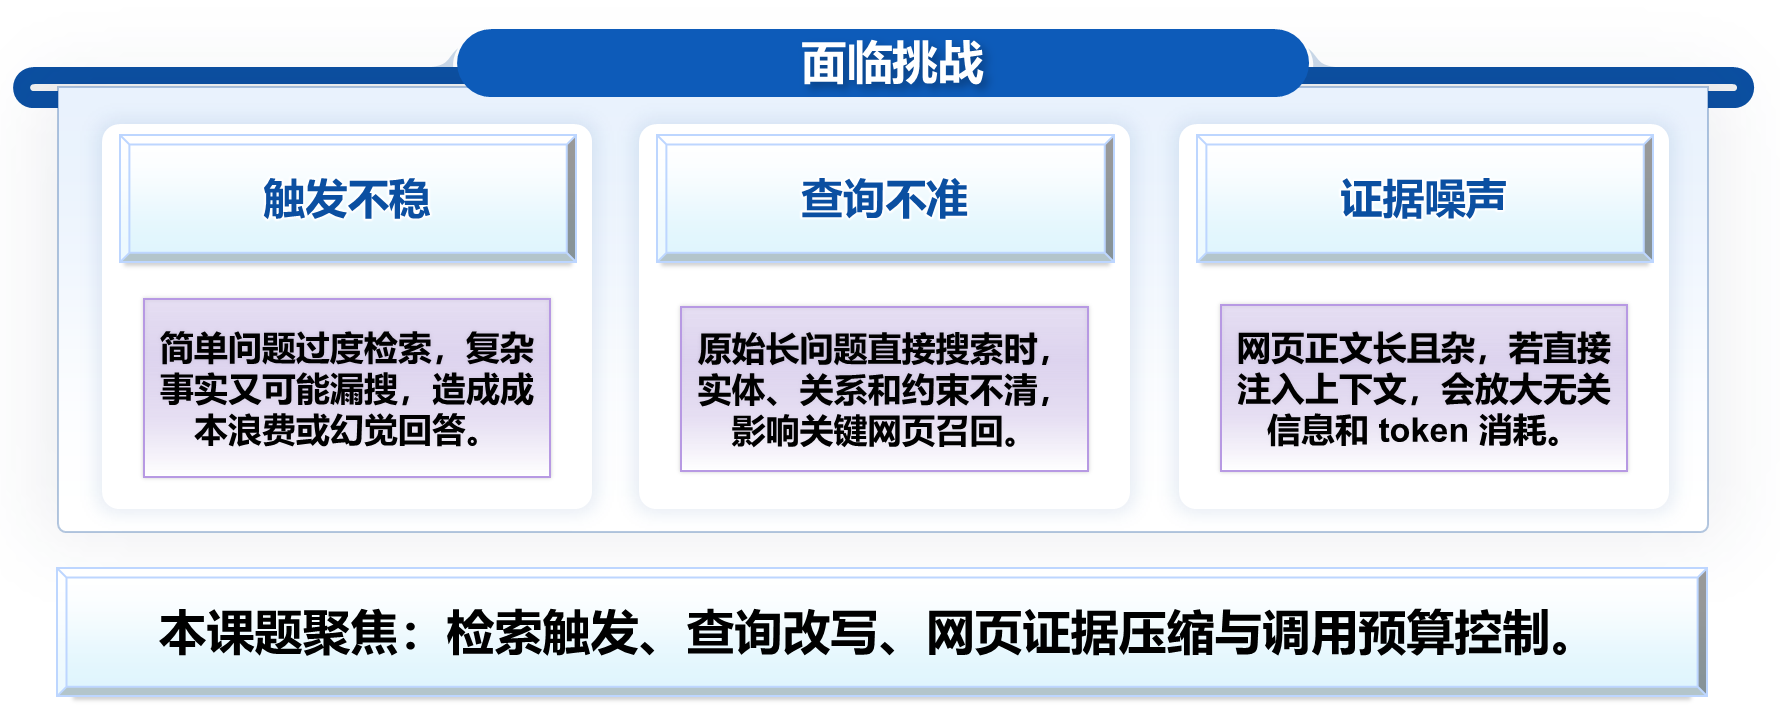
\includegraphics[
        width=1.08\textwidth,
        height=1.08\textheight,
        keepaspectratio
      ]{images/问题分析.png}%
    }
    
\end{frame}
% 基于上面的研究脉络，我把当前开放域问答中的网页检索工具调用问题归纳为三个方面。

% 第一，检索触发不稳定：

% 第一是检索触发不稳定。如果完全让模型自由决定是否调用工具，简单问题可能也会触发搜索，造成过度检索；而真正需要外部证据的问题又可能没有搜索，导致答案缺乏依据甚至出现幻觉。

% 第二，查询质量影响大：

% 第二是查询质量影响大。复杂开放域问题通常不是一个搜索词就能解决的，它可能需要拆成多个中间事实。如果直接把用户的原始长问题丢给搜索引擎，查询可能过长、过泛，导致关键网页召回不足。

% 第三，调用成本需要控制：

% 第三是工具调用成本和响应延迟问题。多轮搜索、网页读取和证据整理都会消耗 token 和时间。如果没有预算控制，系统可能为了一个问题反复搜索、重复读取网页，导致成本和延迟上升。

% 收尾：

% 所以我后面的系统设计主要围绕三个问题展开：什么时候搜、搜什么、搜多少。

\begin{frame}{方法解决的问题}
  \tablebody
  \begin{tabularx}{\textwidth}{B{2.0cm}YP{4.6cm}}
    \toprule
    问题 & 方法设计 & 解决效果 \\
    \midrule
    触发不稳 & 规则信号 + 模型自评，判断时间敏感、长尾事实、多跳关系和证据缺口 & 降低简单问题过度检索，减少复杂问题漏检导致的幻觉回答 \\
    \addlinespace
    查询不准 & 将复杂问题拆成带实体、关系和约束的子查询，并记录检索目的 & 提升关键网页召回质量，避免直接搜索长自然语言问题 \\
    \addlinespace
    证据噪声 & 网页正文抽取后进行证据压缩，输出事实、URL、子目标和相关性评分 & 减少长网页注入造成的噪声和 token 成本，增强答案可追溯性 \\
    \addlinespace
    调用膨胀 & 查询去重、URL 去重、证据去重、最大轮数和 token 预算控制 & 控制搜索次数、读取网页数、响应延迟和 API 成本 \\
    \bottomrule
  \end{tabularx}
  % \vspace{0.5em}
  % \centering
  % {\scriptsize 核心表述：方法解决的不是单点模型能力问题，而是开放域问答中外部信息获取链路不可控的问题。}
\end{frame}

% 相关研究从固定 RAG 发展到智能体式网页检索推理，但在实际开放域问答中，仍然存在检索触发、查询生成、网页证据利用和调用成本控制的问题，因此我的课题围绕网页检索工具调用链路进行系统优化。

\section{研究方案}

\begin{frame}{主要研究内容}
  \centering
  \setlength{\fboxsep}{6pt}
  \researchbox{1. 构建原型系统}{实现开放域问答检索工具调用智能体，支持问题输入、多轮搜索、网页读取、证据整理和答案生成。}
  \hspace{0.04\textwidth}
  \researchbox{2. 设计多轮检索流程}{形成“推理--搜索--阅读--整理--继续推理”的循环，并记录查询、URL、网页片段和使用状态。}

  \vspace{0.85em}

  \researchbox{3. 实现证据压缩模块}{将网页正文转化为短而可验证的结构化证据，包括事实、来源、关联子目标和相关性判断。}
  \hspace{0.04\textwidth}
  \researchbox{4. 开展链路优化评测}{比较直接回答、单次 RAG、多轮检索智能体和改进系统在准确性、效率与稳定性上的差异。}
\end{frame}

\begin{frame}{系统总体架构}
  \centering
  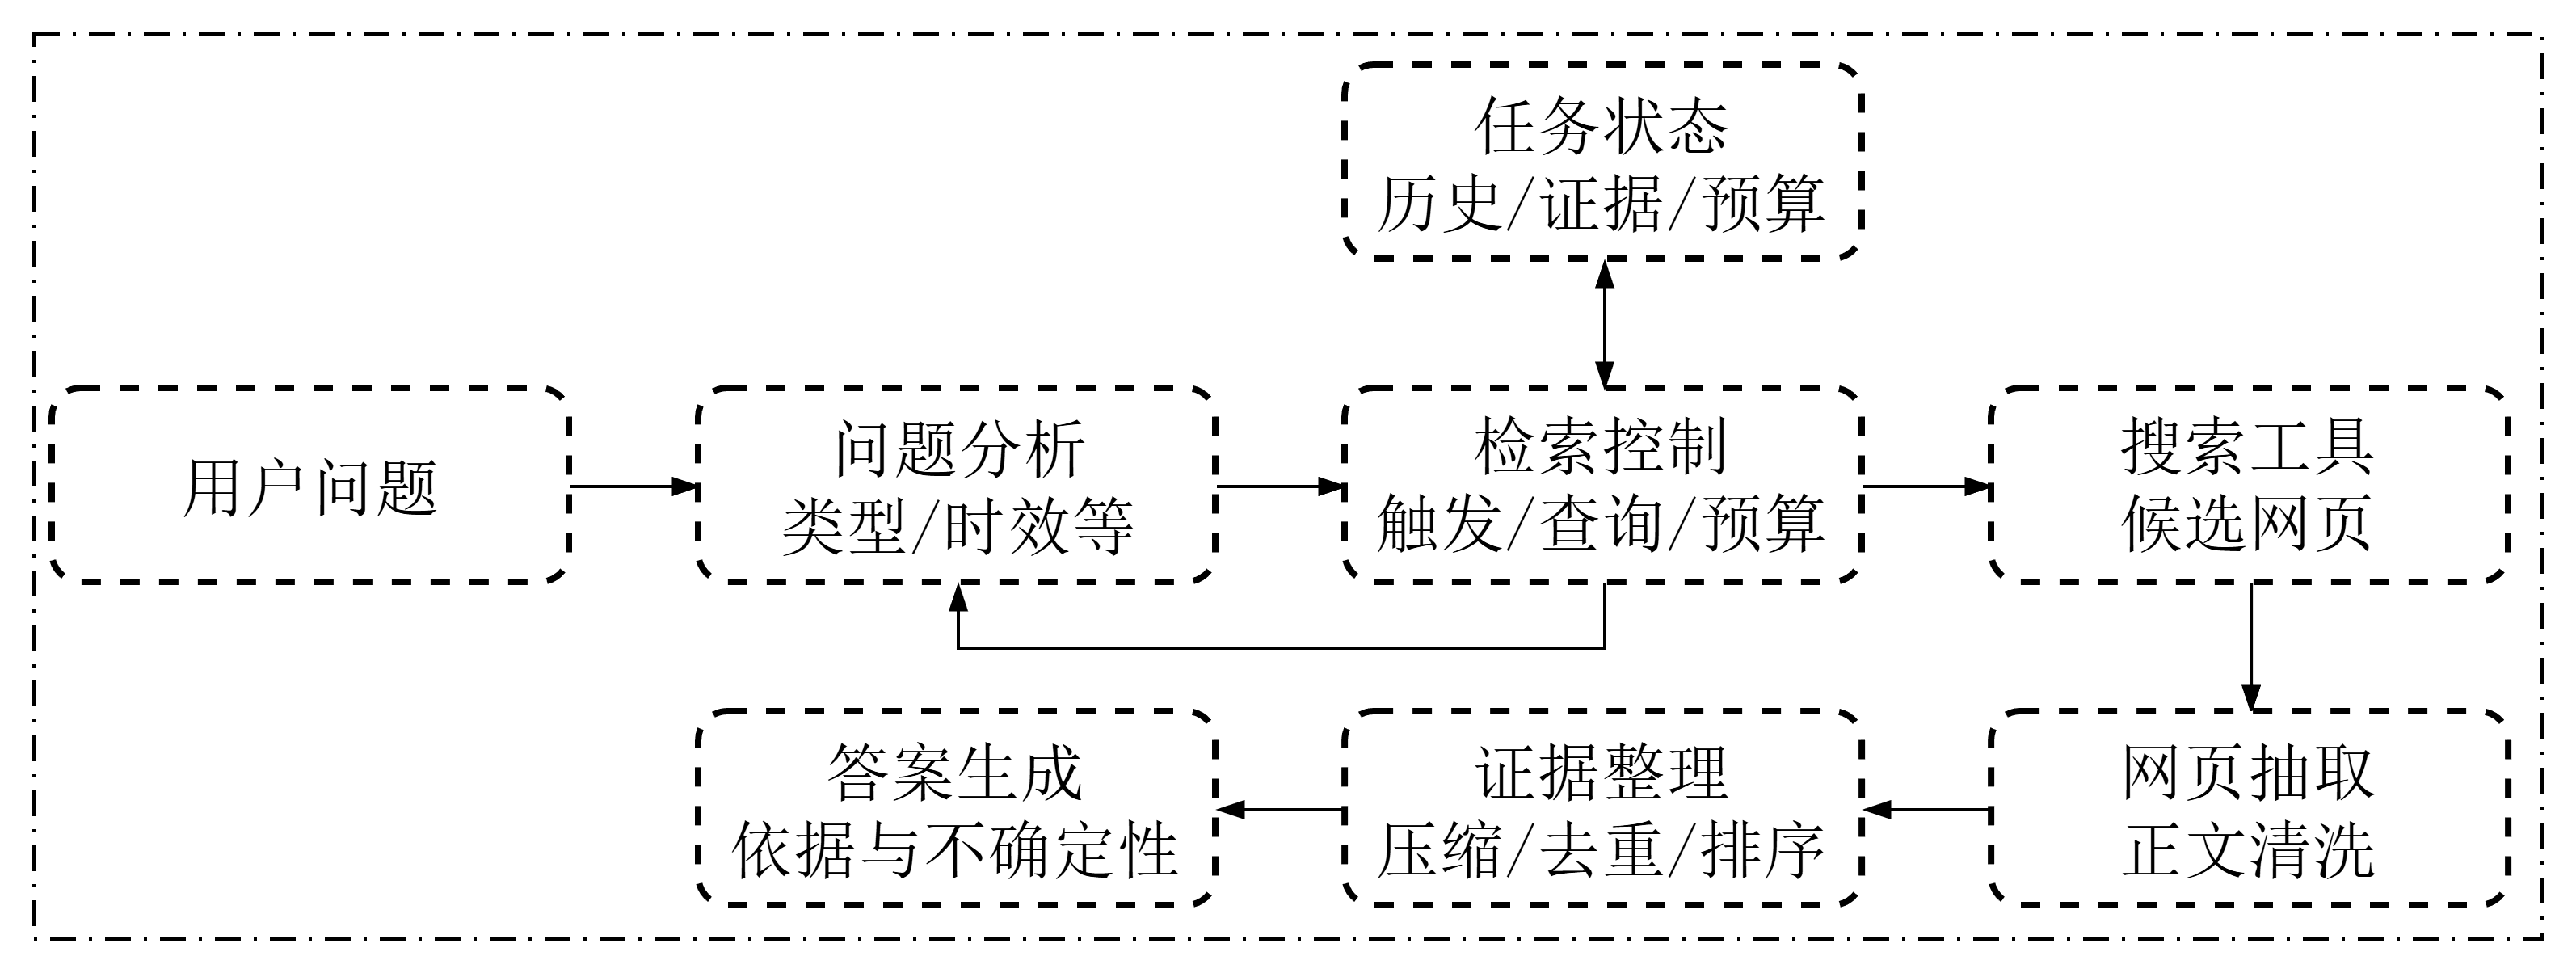
\includegraphics[width=\textwidth,height=0.8\textheight,keepaspectratio]{images/系统.png}

  \vspace{0.2em}
  {\footnotesize 系统以大语言模型为推理核心，围绕网页文本检索工具形成可记录、可控制、可评测的调用链路。}
\end{frame}

% \begin{frame}{模块设计}
%   \tablebody
%   \begin{tabularx}{\textwidth}{B{2.35cm}YP{3.6cm}}
%     \toprule
%     模块 & 主要功能 & 实现方式 \\
%     \midrule
%     问题分析模块 & 识别问题类型、实体、时间敏感性和多跳需求 & 大模型 API + 提示词约束 \\
%     检索控制模块 & 决定是否搜索、生成查询、控制最大轮数和调用预算 & 规则信号 + 模型自评 \\
%     搜索工具模块 & 调用搜索引擎并返回候选结果 & 开放搜索接口，预留替代接口 \\
%     网页抽取模块 & 读取 URL、清洗 HTML、提取正文和标题 & readability / trafilatura / Jina Reader 类工具 \\
%     证据整理模块 & 抽取相关事实、去重、排序、记录来源 & 证据压缩提示词 + 规则整理 \\
%     答案生成模块 & 综合证据生成最终答案并输出依据 & 大模型 API + 结构化证据输入 \\
%     \bottomrule
%   \end{tabularx}
% \end{frame}

\begin{frame}{技术路线}
  \centering

  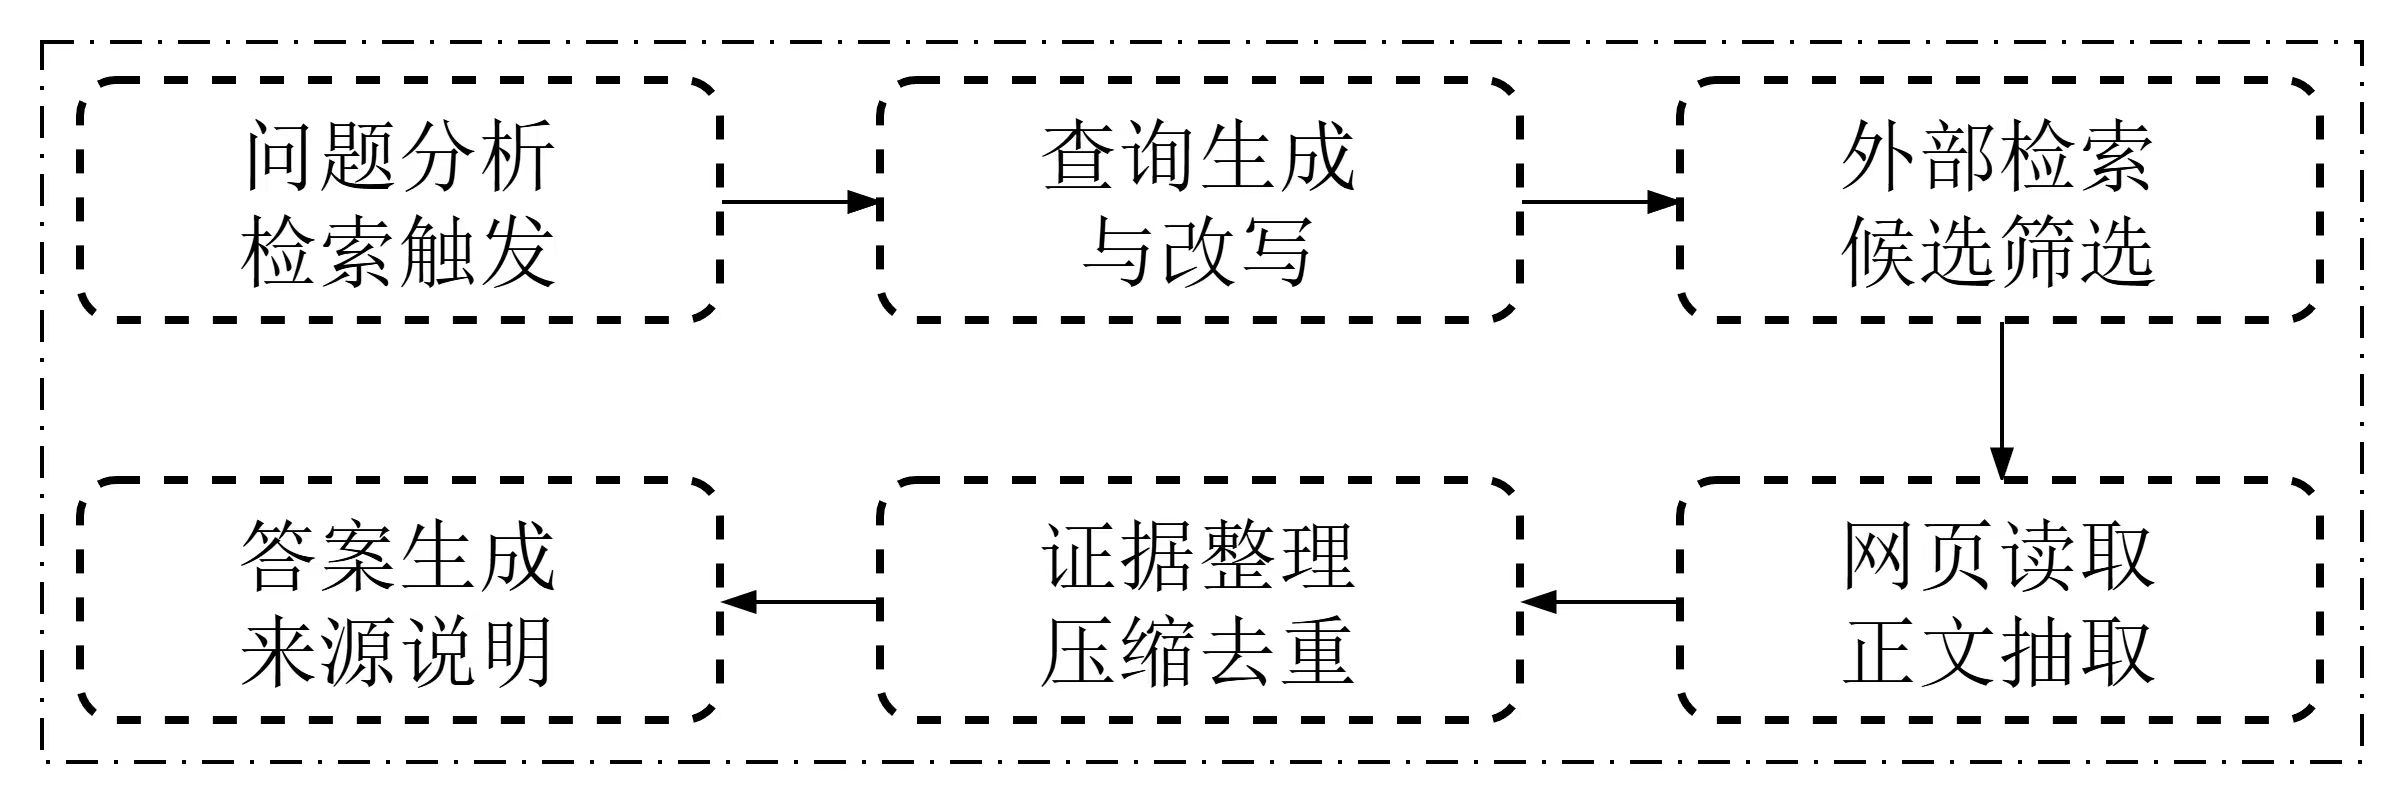
\includegraphics[width=0.96\textwidth,height=0.60\textheight,keepaspectratio]{images/技术路线.jpg}
  \vspace{0.8em}
  
  \smalltag{证据不足时进入下一轮}
  \smalltag{最大轮数}
  \smalltag{最大 URL 数}
  \smalltag{token 预算}
  \smalltag{响应时间与费用记录}
  
  \vspace{0.55em}
  
  {\footnotesize 基本流程覆盖查询生成、外部检索、网页读取、证据整理与答案生成，优化环节贯穿整个调用链路。}
\end{frame}

\section{关键优化}

\begin{frame}{优化一：自适应检索触发}
  \begin{columns}[T]
    \begin{column}{0.48\textwidth}
      \begin{block}{触发信号}
        \begin{itemize}
          \tightlist
          \item 时间表达或最新事实
          \item 长尾实体、专业事实
          \item 多实体比较或多跳关系
          \item 模型自评“缺少证据”
        \end{itemize}
      \end{block}
    \end{column}
    \begin{column}{0.46\textwidth}
      \begin{block}{控制目标}
        \begin{itemize}
          \tightlist
          \item 简单问题尽量直接回答
          \item 复杂事实主动补充外部证据
          \item 通过最大轮数、URL 数和 token 预算限制过度调用
        \end{itemize}
      \end{block}
    \end{column}
  \end{columns}
\end{frame}

\begin{frame}{优化二：查询生成与改写}
  \begin{columns}[T]
    \begin{column}{0.48\textwidth}
      \begin{block}{原始问题}
        \small
        “甲和乙是否出生在同一城市？”
      \end{block}
      \vspace{0.4em}
      \begin{block}{直接搜索的问题}
        \small
        查询过长、意图混合，容易召回泛化页面或问答噪声。
      \end{block}
    \end{column}
    \begin{column}{0.46\textwidth}
      \begin{block}{改写策略}
        \begin{itemize}
          \tightlist
          \item 明确每个查询的检索目的
          \item 拆分为关键实体 + 关系词
          \item 保留必要时间、地点和限定条件
        \end{itemize}
      \end{block}
      \vspace{0.4em}
      \smalltag{甲 birth place}
      \smalltag{乙 birth place}
    \end{column}
  \end{columns}
\end{frame}

\begin{frame}{优化三：网页证据压缩}
  \begin{columns}[T]
    \begin{column}{0.45\textwidth}
      \begin{block}{输入}
        \begin{itemize}
          \tightlist
          \item 当前问题与子目标
          \item 搜索查询与网页 URL
          \item 网页标题、摘要、正文片段
          \item 已有推理状态
        \end{itemize}
      \end{block}
    \end{column}
    \begin{column}{0.49\textwidth}
      \begin{block}{输出结构}
        \begin{tabular}{@{}ll@{}}
          \kw{fact} & 可验证事实 \\
          \kw{url} & 来源链接 \\
          \kw{goal} & 支持的子问题 \\
          \kw{time} & 证据时间 \\
          \kw{score} & 相关性评分 \\
        \end{tabular}
      \end{block}
      \vspace{0.4em}
      {\footnotesize 目标：让主模型接收短证据，而不是整篇网页。}
    \end{column}
  \end{columns}
\end{frame}

\begin{frame}{优化四：冗余调用与预算控制}
  \begin{center}
    \begin{tikzpicture}[
      flowstep/.style={draw=sintefblue, rounded corners=2pt, minimum width=2.8cm,
      minimum height=.8cm, align=center, font=\footnotesize},
      arrow/.style={-{Latex[length=2mm]}, draw=sintefblue, line width=.55pt}
    ]
      \node[flowstep] (a) {查询去重};
      \node[flowstep, right=0.7cm of a] (b) {URL 去重};
      \node[flowstep, right=0.7cm of b] (c) {证据去重};
      \node[flowstep, below=0.75cm of b] (d) {新增证据价值判断};
      \node[flowstep, below=0.75cm of d] (e) {达到预算或证据充分时停止};

      \draw[arrow] (a) -- (b);
      \draw[arrow] (b) -- (c);
      \draw[arrow] (b) -- (d);
      \draw[arrow] (c) -- (d);
      \draw[arrow] (d) -- (e);
    \end{tikzpicture}
  \end{center}
  \vspace{0.3em}
  \centering
  \smalltag{平均搜索次数}
  \smalltag{平均读取网页数}
  \smalltag{token 消耗}
  \smalltag{响应时间}
  \smalltag{API 成本}
\end{frame}

% 这一页是冗余调用与预算控制模块。它主要解决工具调用成本和响应延迟问题。系统首先对模型生成的 query 做去重，避免重复搜索；然后对搜索结果 URL 去重，避免重复读取同一网页；接着对抽取到的证据片段进行去重，判断当前搜索是否带来了新的有效证据。如果连续搜索没有新增证据，或者证据已经足够支持答案，系统就提前停止。同时系统设置最大搜索轮数、最大读取网页数和 token 预算，用来控制整体成本。最后我会用平均搜索次数、读取网页数、token 消耗、响应时间和 API 成本来评估这个模块的效果。

\section{实验与计划}

\begin{frame}{实验方案}
  \begin{columns}[T]
    \begin{column}{0.47\textwidth}
      \begin{block}{数据来源}
        \begin{itemize}
          \tightlist
          \item HotpotQA：多跳实体关系推理
          \item MuSiQue / 2WikiMultiHopQA：组合问答
          \item GAIA：真实信息获取与工具使用
          \item WebWalkerQA：网页检索与多步定位
          % \item 自建网页文本问题集
        \end{itemize}
      \end{block}
    \end{column}
    \begin{column}{0.47\textwidth}
      \begin{block}{对比方法}
        \begin{itemize}
          \tightlist
          \item Direct LLM：不检索直接回答
          \item Standard RAG：原始问题单次检索
          \item Agentic Search：多轮搜索，无独立证据压缩
          \item Ours：加入触发、改写、压缩和预算控制
        \end{itemize}
      \end{block}
    \end{column}
  \end{columns}
\end{frame}

\begin{frame}{评价指标}
  \centering
  \tablebody
  \begin{tabularx}{\textwidth}{B{2.35cm}Y}
    \toprule
    指标类别 & 具体度量 \\
    \midrule
    答案准确性 & Exact Match、F1 \\
    检索有效性 & 支持答案网页命中率、有效证据占比、证据相关性 \\
    工具调用效率 & 平均搜索次数、平均读取网页数、响应时间、token 消耗、API 费用 \\
    推理稳定性 & 同一问题多次运行的答案一致性、证据一致性和失败率 \\
    可解释性 & 最终答案是否能对应明确证据来源，是否存在无证据断言 \\
    \bottomrule
  \end{tabularx}
\end{frame}

% \begin{frame}{进度安排}
%   \scriptsize
%   \begin{tabularx}{\textwidth}{>{\bfseries}p{2.5cm}X}
%     \toprule
%     时间 & 主要任务 \\
%     \midrule
%     2026年4月下旬 & 完成开题报告；阅读 RAG、ReAct、WebGPT、IRCoT 与网页信息获取相关论文，明确系统边界和指标。 \\
%     2026年5月上旬 & 搭建基础原型，实现大模型 API、开放搜索接口、网页正文抽取和单轮 RAG 回答流程。 \\
%     2026年5月中旬 & 完成多轮检索 Agent 主循环，实现检索历史、证据缓存、调用预算和异常处理。 \\
%     2026年5月下旬 & 实现文档推理与证据压缩、查询改写、证据排序去重和主要优化方法。 \\
%     2026年6月上旬 & 完成公开数据集子集和自建问题集实验，统计准确率、F1、调用次数、延迟和成本。 \\
%     2026年6月中旬 & 完成实验分析、案例分析、论文初稿和系统代码整理，准备毕业答辩材料。 \\
%     \bottomrule
%   \end{tabularx}
% \end{frame}

\begin{frame}{预期成果与风险应对}
  \begin{columns}[T]
    \begin{column}{0.48\textwidth}
      \begin{block}{预期成果}
        \begin{itemize}
          \tightlist
          \item 可运行的开放域问答工具调用智能体原型
          \item 可复现实验脚本与评测数据子集
          \item 至少一种关键优化方法及消融实验
          \item 实验结果表、案例分析和毕业论文
        \end{itemize}
      \end{block}
    \end{column}
    \begin{column}{0.46\textwidth}
      \begin{block}{风险应对}
        \begin{itemize}
          \tightlist
          \item 搜索接口：缓存、重试和备用接口
          \item 网页噪声：长度、重复度、关键词覆盖过滤
          \item 触发不稳：规则信号 + 模型自评 + 预算限制
          % \item 评价主观：公开指标 + 人工核验表
        \end{itemize}
      \end{block}
    \end{column}
  \end{columns}
\end{frame}

\begin{frame}{总结}
  \begin{center}
    \large
    本课题面向开放域问答中的外部知识获取需求，\\[0.4em]
    设计一个可运行、可控制、可评测的\\[0.4em]
    \kw{网页检索工具调用智能体}。
  \end{center}
  \vspace{1em}
  \begin{columns}[T]
    \begin{column}{0.31\textwidth}
      \centering
      \kw{系统实现}\\
      {\small 多轮检索与网页阅读流程}
    \end{column}
    \begin{column}{0.31\textwidth}
      \centering
      \kw{链路优化}\\
      {\small 触发、查询、证据、预算}
    \end{column}
    \begin{column}{0.31\textwidth}
      \centering
      \kw{实验评测}\\
      {\small 准确性、效率、稳定性}
    \end{column}
  \end{columns}
\end{frame}

\backmatter

\end{document}
